\PassOptionsToPackage{dvipsnames}{xcolor}
\documentclass[a4paper,11pt]{book}
\usepackage[]{geometry}

\usepackage{ucs}
\usepackage[utf8]{inputenc}
\usepackage{amsmath}
\usepackage{amssymb}
\usepackage{siunitx}
\usepackage{cancel}
\usepackage[italian]{babel}
\usepackage{fontenc}
\usepackage{graphicx}
\graphicspath{{img/}}
\usepackage{circuitikz}
\ctikzset{
    resistors/scale=0.7,
    capacitors/scale=0.7,
    inductors/scale=0.7,
    sources/scale=0.7
    }

\usepackage{float}
\usepackage{xcolor}

\usepackage{hyperref}

%Definizione 'globale' larghezza immagini
\newcommand{\picwid}{0.3\linewidth}

\date{28/11/21}
\title{Appunti Elementi di Automatica}
\author{Daniele Olivieri}
\begin{document}
\maketitle
\tableofcontents
%Lezione 01
\chapter{Introduzione}
L'automazione è una disciplina estremamente ampia, si intende in questo corso con
\textit{automazione} la progettazione, la realizzazione e la gestione di sistemi in grado di
eseguire dei compiti in maniera autonoma, senza l'intervento dell'uomo.

Nel corso verranno effettuate le analisi di sistemi dinamici, con un focus finale sulle analisi di
sistemi di controllo che verranno approfondite al corso di ``controlli''.

L'uomo ha sempre cercato di automatizzare i processi o i compiti che doveva eseguire, per ridurre
la fatica e l'usura per le attività manuali.

Un esempio è il \textbf{regolatore di Watt}, una macchina in grado di regolare il grado di
ammissione di una valvola di alimentazione per una macchina a vapore, al fine di mantenere costante
la velocità di rotazione della macchina.

Inizialmente l'operazione era compiuta da un operatore che regolava la temperatura della caldaia
fornendo più o meno combustibile.

Quest'oggetto racchiude l'essenza dei controlli automatici:
\begin{itemize}
 \item Elemento di trasduzione e misura, fondamentale per ottenere informazioni sulla grandezza da
controllare, in questo caso la velocità di rotazione delle macchine da controllare. L'uscita dello
strumento di misura può essere di diversa natura rispetto alla grandezza misurata ma comunque
proporzionale ad esso.
 \item Elemento di controllo (controllore), in questo caso il sistema di leve e pesi che varia la
posizione del cursore in funzione dell'input e delle sue caratteristiche come i pesi e le lunghezze
delle leve.
\item Attuatore, ossia uno strumento in grado di attuare la decisione del controllore sul sistema,
nel caso precedente la valvola.
\end{itemize}

Nel contesto più generale dei sistemi dinamici si riuscirà a modellare ed analizzare i sistemi
dinamici in generale e comprendere le proprietà fondamentali e strutturali dei sistemi studiati.

\section{Sistemi dinamici}
Un sistema è qualunque oggetto o processo materiale o immateriale, ben delimitato nel suo
funzionamento.
Potrebbe essere un sistema meccanico o termico, o ad esempio un sistema immateriale come
l'andamento del PIL in Italia.

Gli oggetti di interesse in particolare sono quelli \textit{dinamici}
che hanno ossia la possibilità di variare nel tempo alcune grandezze che li caratterizzano.

L'unica variabile indipendente considerata nell'intero corso sarà il tempo, anche i sistemi
astratti saranno comunque sistemi ``esistenti''.

33:04

%lezione_02.tex
\chapter{Modelli di sistemi dinamici}
I principali modelli di sistemi dinamici sono due:
\begin{itemize}
\item [$(IU)$]Ingresso-uscita
\begin{equation}
f\left(y^{(n)},y^{(n-1)},\ldots,y,u^{(m)},u^{(m-1)},\ldots,u\right)=0
\label{eq.:modello_ingresso_uscita}
\end{equation}
con $m<n$ (per la regola di Cauchy) per avere un sistema strettamente causale. Con $m=n$ un sistema
è causale ma non strettamente causale, in genere tutti i modelli fisici sono strettamente causali.
La \ref{eq.:modello_ingresso_uscita} prende il nome di \textit{equazione generale del sistema}
mentre $n$
prende il nome di \textit{ordine del sistema}.
La funzione può anche essere un sistema di equazioni differenziali di ordine inferiore.
\item[$(ISU)$] Ingresso-stato-uscita
\begin{equation}
y(t) = x_1(t), \dot{y}(t) = x_2(t),\ldots,y^{(n-1)}(t)=x_n(t)
\label{eq.:modello_ingresso_stato_uscita}
\end{equation}
Compaiono in questo modello tre tipologie di variabili, \textit{ingresso} e \textit{uscita} come nel
caso precedente e le variabili \textit{di stato} necessarie a completare il problema di Cauchy.
Un possibile insieme di variabili di stato sono quelle necessarie a specificare le condizioni
iniziali dell'equazione differenziale. Questo insieme può essere definito come \textit{stato} del
sistema.
Nella \ref{eq.:modello_ingresso_stato_uscita} si vede che il numero di variabili di stato $(x_n)$
necessarie alla risoluzione del problema è pari all'ordine del sistema.
\end{itemize}

Qualunque sistema dinamico può essere rappresentato con una diversa scelta delle variabili di
stato, varieranno le equazioni ma il modello resta valido per quel determinato sistema. La
rappresentazione ingresso-uscita è invece unica.

Si vede che nella rappresentazione $ISU$, una volta ottenuta l'equazione del sistema, questa può
essere trasformata per evidenziare particolari proprietà del sistema.

\newpage
\section{Costruzione di un modello ISU}
Si può costruire seguendo quattro passaggi
\begin{enumerate}
\item Scrivere tutte le equazioni del sistema (eq. diff.) conoscendo il modello fisico del sistema
\item Individuare le variabili d'ingresso e uscita, mediante il principio di causalità
\item Scegliere le variabili di stato dopo averne individuato il numero. Una scelta possibile è
quella mediante la regola di Cauchy
\item Riscrivere le equazioni di partenza trovate al punto uno nella seguente forma
\begin{equation}\left\{ \begin{aligned}
&\dot{x}_1 = f_1\left(x_1,\ldots,x_n,u_1,\ldots,u_m,t\right)\\
&\ \vdots \qquad \vdots\\
&\dot{x}_n = f_n\left(x_1,\ldots,x_n,u_1,\ldots,u_m,t\right)\\
&y_1 = g_1\left(x_1,\ldots,x_n,u_1,\ldots,u_m,t\right) \\
&\ \vdots \qquad \vdots\\
&y_n = g_n\left(x_1,\ldots,x_n,u_1,\ldots,u_m,t\right)
\end{aligned}\right.\qquad\text{ISU}
\label{eq.:ISU_generale}
\end{equation}
la $t$ in questo caso indica l'eventuale tempo varianza dei parametri del sistema e non la
dipendenza dal tempo delle variabili di stato (assunta vera implicitamente).
\end{enumerate}

\subsection{Costruzione modello ISU RLC}
Si considera l'esempio mostrato in figura \ref{Fig.:circuito_RLC}, analizzando l'equazione
\ref{eq.:ISU_generale} si vede che sono presenti $n$ equazioni differenziali di primo grado dato
che le funzioni $f$ e $g$ sono equazioni algebriche, non contengono termini differenziali.
Sono invece presenti $p$ equazioni puramente algebriche $g$ che legano lo stato, l'ingresso, il
tempo alle uscite.

\begin{enumerate}
\item Ricordando l'equazione del sistema ricavata in \ref{eq:equazione_RLC}
si formalizza il modello
\begin{equation}\left\{
\begin{aligned}
 e &= R i + L\dot{i} + \frac{q}{C}\\
 i &= \dot{q}
\end{aligned}\right.\end{equation}
\item Si individuano tutte le variabili: $e,i,q$

Si individuano dunque le variabili d'ingresso tra quelle con ordine di derivata più basso, in
questo caso la $e$ è differenziata zero volte, sarà un ingresso, in questo caso l'unico; le altre,
differenziate una volta, saranno le potenziali variabili di uscita.
\item Si scelgono le variabili di stato, si deve prima determinare l'ordine del sistema:\newline
\emph{il
numero di variabili di stato è pari alla somma del numero di volte che le variabili delle equazioni
compaiono differenziate tolte le variabili d'ingresso.}

Sommando l'ordine di derivazione di $i$ e $q$, variabili non d'ingresso si ottiene dunque $n=2$.

\item Si possono scegliere come variabili di stato tutte quelle che determinano le condizioni
iniziali, ossia\newline
\emph{tutte le variabili che compaiono differenziate e in numero pari al numero di volte
in cui viene differenziata.}

Per il sistema in esame
$$
x_1 = q,\quad x_2 = i
$$
\item Scrittura delle equazioni in forma ISU

$$
\left\{\begin{aligned}
\dot{x}_1 &= f_1\left(x_1,x_2,u\right) = \dot{q} = i = x_2\\
\dot{x}_2 &=f_2(x_1,x_2,u) = \dot{i} = \frac{e}{L} - \frac{R}{L}i-\frac{1}{LC}q =\\
&= -\frac{1}{LC}x_1 - \frac{R}{L}x_2 + \frac{1}{L}u\\
y_1 &= i = g_1(x_1,x_2,u)=x_2\\
y_2 &=q = g_2(x_1,x_2,u)=x_1
\end{aligned}\right.
$$
\end{enumerate}

\newpage
\section{Classificazione dei sistemi dinamici}
Per comodità si riporta la \ref{eq.:ISU_generale} in forma più compatta.
Si costruisce un vettore di variabili di stato, d'ingressi e di uscite
$$
x = \begin{bmatrix}
x_1\\
x_2\\
\vdots\\
x_n
\end{bmatrix} \in \mathbb{R}^n \textcolor{red}{\left(\in\mathbb{C}^n\right)}\
u=\begin{bmatrix}
u_1\\
u_2\\
\vdots\\
u_m
\end{bmatrix}\in\mathbb{R}^m\
y=\begin{bmatrix}
y_1\\
y_2\\
\vdots\\
y_p
\end{bmatrix}\in \mathbb{R}^p
$$
l'esistenza di variabili complesse per le variabili di stato è giustificata da scelte pratiche
utili alla risoluzione del problema anche se non legate strettamente a fenomeni fisici.

Di conseguenza la $f$ sarà un vettore di funzioni
$$\left.\begin{aligned}
&f_1\left(x_1,...,x_n,u_1,...,u_m,t\right)=f_1(x,u,t)\\
&\ \vdots\\
&f_n\left(x_1,\ldots,x_n,u_1,\ldots,u_m,t\right)=f_n(x,u,t)
\end{aligned}\right\} \Rightarrow f(x,u,t)=\begin{bmatrix}
f_1(x,u,t)\\
\vdots\\
f_n(x,u,t)
\end{bmatrix}
$$
Analogamente per le funzioni $g$
$$
\left.\begin{aligned}
&g_1(x,u,t)\\
&\ \vdots\\
&g_p(x,u,t)
\end{aligned}\right\}\Rightarrow
g(x,u,t) = \begin{bmatrix}
g_1(x,u,t)\\
\vdots\\
g_p(x,u,t)
\end{bmatrix}
$$

La forma generale della ISU diventa
\begin{equation}\text{ISU }\left\{
\begin{aligned}
\dot{x} = f(x,u,t)\\
y = g(x,u,t)
\end{aligned}\right.
\label{eq.:ISU_compatta}
\end{equation}

Si suppone che le funzioni $f,g$ siano lineari in $x$ e $u$ ossia che possano essere espresse come
combinazione lineare di quelle variabili $(x,u)$.

Ad esempio la funzione $f$
$$\begin{aligned}
&\dot{x}_1 = a_{11}(t)x_1+a_{12}(t)x_2 + \ldots + a_{1n}(t)x_n + b_{11}(t)u_1+\ldots+b_{1m}(t)u_m\\
&\ \vdots\\
&\dot{x}_n = a_{n1}(t)x_1 +  a_{n2}(t)x_2 + \ldots + a_{nn}(t)x_n + b_{n1}(t)u_1+\ldots+b_{nm}(t)u_m
\end{aligned}
$$

Analogamente la funzione $g$
$$\begin{aligned}
&g_1 = c_{11}(t)x_1 + \ldots + c_{1n}(t)x_n + d_{11}(t)u_1 + \ldots + d_{1m}(t)u_m\\
&\ \vdots\\
&g_p = c_{p1}(t)x_1 + \ldots + c_{pn}(t)x_n + d_{p1}(t)u_1+\ldots+d_{pm}(t)u_m
\end{aligned}$$

Si può scrivere il sistema in forma vettoriale ottenuto dal prodotto di un vettore riga contenente
i coefficienti e un vettore colonna contenente le variabili, questo per ogni elemento di
$\dot{x}$, si ottiene dunque una matrice $n\times n$ di coefficienti ed un vettore colonna di
variabili $x$.
$$\begin{aligned}
f = \dot{x} = A \cdot x + B\cdot u
\end{aligned}
$$
con
$$
A = \begin{bmatrix}
a_{11} & \dots & a_{1n} \\
\vdots & \ddots & \vdots \\
a_{n1} & \dots & a_{nn}
\end{bmatrix} \in \mathbb{R}^{n\times n} \quad
B = \begin{bmatrix}
b_{11} & \dots & b_{1m} \\
\vdots & \ddots & \vdots \\
b_{n1} & \dots & b_{nm}
\end{bmatrix} \in \mathbb{R}^{n\times m}
$$
La matrice $A$ è sempre quadrata mentre la matrice $B$ ha una dimensione che dipende dal numero di
ingressi e può diventare un vettore se l'ingresso è unico.

Si ripete la procedura per le funzioni $g$
$$
g = y = C\cdot x + D\cdot u
$$
con
$$
C = \begin{bmatrix}
c_{11} & \dots & c_{1n} \\
\vdots & \ddots & \vdots \\
c_{p1} & \dots & c_{pn}
\end{bmatrix} \in \mathbb{R}^{p\times n} \quad
D = \begin{bmatrix}
d_{11} & \dots & d_{1m} \\
\vdots & \ddots & \vdots \\
d_{p1} & \dots & d_{pm}
\end{bmatrix} \in \mathbb{R}^{p\times m}
$$
La matrice $D$ diventa uno scalare se il sistema ha un solo ingresso e una sola uscita.

Riassumendo
\begin{equation}
\text{ISU } \left\{\begin{aligned}
\dot{x} &= A(t)x + B(t) u \\
y &= C(t) x + D(t) u
\end{aligned}\right.
\label{eq.:ISU_compatta_matrice}
\end{equation}
\emph{Un sistema si dice \textbf{lineare} se le funzioni $f$ e $g$ sono entrambe lineari nello stato
e nell'ingresso},
ossia se possono essere scritte nella forma \ref{eq.:ISU_compatta_matrice}.

Se le equazioni del sistema compaiono nella seguente forma
$$\left\{\begin{aligned}
\dot{x} &= f(x,u)\\
y &= g(x,u)\end{aligned}\right.
$$
allora il sistema si dice \textit{stazionario} o \textit{tempo invariante},
ossia il sistema avrà sempre la stessa evoluzione fissato l'ingresso e lo stato iniziale. In caso
contrario il sistema si comporterebbe in maniera differente a seconda di quando viene
sollecitato e analizzato.
Se il sistema gode di entrambe le proprietà si dirà \textit{Lineare Tempo Invariante} e saranno
quelli prevalentemente analizzati nel corso, sono sempre risolvibili.
\newpage
\subsection{Ulteriori classificazioni}
Nel seguente sistema, l'uscita non dipende \textit{direttamente} dall'ingresso
$$
\left\{\begin{aligned}
\dot{x} &= f(x,u,t) \\
y &= g(x,t)
\end{aligned}
\right.
$$
viene definito \emph{sistema strettamente proprio}, in caso contrario è \emph{proprio}.

Nel caso di sistemi lineari
$$
\left\{
\begin{aligned}
\dot{x} &= Ax + Bu \\
y &= Cx
\end{aligned}
\right. \qquad D = 0 \Leftrightarrow \text{Strettamente proprio}
$$
In natura esistono solo sistemi strettamente propri, non esistono quelli propri,
qualunque ingresso ha bisogno di propagarsi nel sistema entro un certo tempo, non può quindi
modificare l'uscita istantaneamente.

\section{Sistemi elettrici}
Si richiamano le convenzioni utilizzate nei sistemi elettrici, saranno composti da uno o più
generatori di tensione o corrente e composti da bipoli passivi.

Verrà utilizzata la convenzione dell'utilizzatore per i seguenti bipoli
\begin{figure}[h]
\centering
\begin{circuitikz}
\draw (0,2) [R=$R$,i>^=$i$,v<=$v$] to (0,0);
\draw (1.5,1) node[label]{$v = Ri$};
\draw (4,2) [C=$C$,i>^=$i$,v<=$v$] to (4,0);
\draw (5.8,1) node[label]{$q = Cv$};
\draw (7.5,2) [L=$L$,i>^=$i$,v<=$v$] to (7.5,0);
\draw (9,1) node[label]{$\Phi = Li$};
\end{circuitikz}
\end{figure}

Derivando le equazioni dei bipoli dinamici rispetto al tempo si ottiene
$$\begin{aligned}
q &= Cv\stackrel{\frac{d}{dt}}{\rightarrow} \frac{dq}{dt} = i =
\frac{d}{dt} \left(Cv\right) \stackrel{C\text{ cost}}{=} C\frac{dv}{dt} = C\dot{v}\\
\Phi &= Li \stackrel{\frac{d}{dt}}{\rightarrow} \frac{d\Phi}{dt} = v = \frac{d}{dt}\left(Li \right)
\stackrel{L\text{ cost}}{=} L \frac{di}{dt} = L \dot{i}
\end{aligned}$$

Si aggiungono ai bipoli passivi i generatori di tensione e corrente
\begin{figure}[h]
\centering
\begin{circuitikz}[american voltages]
\draw (0,0) [european voltage source] to (0,2);
\draw (0.5,2) to [open, v^>=$ $,l=$e$] (0.5,0);
\draw (4,2) [current source,i<^=$i$] to (4,0);
\end{circuitikz}
\end{figure}

\subsection{Esempio rete RLC}
Si ha la seguente rete
\begin{figure}[h]
\centering
\begin{circuitikz}
\draw (0,0) to [voltage source,v=$e$]  (0,2)
            to [L=$L$,i>^=$i_L$,-*] (2,2)  node[above,label]{$A$}
            to [C,l_=$C$,i>_=$i_C$] (2,0)
            to (0,0);
\draw (2,2) to (3,2) to [R=$R$,i>^=$i_R$] (3,0) to (2,0);
\end{circuitikz}
\end{figure}

Si ricavano le equazioni del sistema utilizzando in questo caso le leggi di Kirchhoff applicate al
nodo $A$ e alla prima maglia (che comprende il generatore)
$$\left\{\begin{aligned}
i_L &= i_C + i_R &\Rightarrow&\ i_L = C\dot{v}_C + \frac{v_C}{R}\\
e &= v_L + v_C &\Rightarrow&\ e = L\dot{i}_L + v_C\\
v_C &= v_R
\end{aligned}\right.
$$

Elaborando le equazioni si vede che alcune variabili potranno risultare superflue, ad esempio in
questo caso $v_C$ e $v_R$ sono la stessa grandezza.

Si individuano ora le variabili e si dividono in ingressi e uscite al fine di rispettare il
principio di causalità ricordando che gli ingressi compaiono differenziati un numero minore di volte
$$\begin{matrix}
e& i_L& v_C\\
(0) & (1) & (1)\\
u & y & y\\
u & x_1 & x_2
\end{matrix}
$$

Si scelgono le variabili di stato, applicando la legge di Cauchy, il numero di ingressi è pari a
due perché entrambe le variabili compaiono differenziate una sola volta.
$$
n=2,\ x_1 = i_L,\ x_2 = v_C
$$

Si scrive quindi la ISU (il sistema è tempo invariante quindi le funzioni della ISU non dipendono
da $t$
$$\begin{aligned}
\dot{x}_1 &= f_1(x_1,x_2,u) = \dot{i}_L = \frac{e}{L} - \frac{v_C}{L} = -\frac{1}{L}x_2 +
\frac{1}{L} u\\
\dot{x}_2 &= f_2(x_1,x_2,u) = \dot{v}_C = \frac{i_L}{C} - \frac{v_C}{RC} = \frac{1}{C}x_1 -
\frac{1}{RC}x_2
\end{aligned}$$

Andrebbero aggiunte le relazioni che legano le uscite all'effettiva variabile di studio ad esempio
la tensione ai capi della resistenza e la corrente nell'induttanza, dunque
$$
y_1 = v_R,\ y_2 = i_L
$$
ma riferendosi al modello ISU
$$\begin{aligned}
y_1 &= g_1(x_1,x_2,\cancel{u}) = v_R = v_C = x_2\\
y_2 &= g_2(x_1,x_2,\cancel{u}) = i_L = x_1
\end{aligned}$$

Si vuole ora classificare la ISU, si verifica la linearità, tutte le funzioni $f$ e $g$ sono
lineari nello stato e negli ingressi, di conseguenza il sistema è lineare, è anche tempo invariante
dato che i parametri del sistema sono costanti nel tempo.

Si afferma ora che il sistema è strettamente proprio, ossia nell'espressione della $g$
non compare l'ingresso $u$.

Si riscrive il sistema in forma compatta utilizzando la notazione
\ref{eq.:ISU_compatta_matrice} ponendo
$$\begin{aligned}
x &= \begin{pmatrix}x_1\\x_2 \end{pmatrix},& u &= \begin{pmatrix} u \end{pmatrix},&
y&=\begin{pmatrix}
y_1 \\y_2 \end{pmatrix}\\
n&=2& m&=1&  p&=2
\end{aligned}
$$
dunque
\begin{equation}\left\{\begin{aligned}
&\dot{x} = \begin{bmatrix}
0 & -\frac{1}{L}\\
\frac{1}{C} & -\frac{1}{RC}
\end{bmatrix} x + \begin{bmatrix}\frac{1}{L}\\0 \end{bmatrix} u\\
&y =\begin{bmatrix}
0 & 1\\
1 & 0
\end{bmatrix} x + \begin{bmatrix}0\\0 \end{bmatrix}u
\end{aligned}\right.\end{equation}
\newpage

\subsection{Esempio rete RLC 2}
Si analizza il seguente circuito
\begin{figure}[h]
\centering
\begin{circuitikz}
\draw (0,0) to [current source,i=$i_1$] (0,2) to (2,2) node[above,label]{$A$}
            to [R=$R_1$,i>_=$i_{R_1}$,v<=$v_1$,*-] (2,0) to (0,0);
\draw (2,2) to (4,2) to [C=$C_1$,i>_=$i_{C_1}$] (4,0) to (2,0);
\draw (4,2) to [L=$L$,i>^=$i_L$] (6,2)
            to [C=$C_2$,i>^=$i_{C_2}$,v<=$v_{C_2}$] (6,0) to (4,0);
\draw (6,2) to (8,2) node[above,label]{$B$} to [R=$R_2$,i>^=$i_{R_2}$,*-] (8,0) to (6,0);
\draw (8,2) to (10,2) to [current source,i>^=$i_2$] (10,0) to (8,0);
\end{circuitikz}
\end{figure}

Applicando le leggi di Kirchhoff
$$\begin{aligned}
A: i_1 &= i_{R_1} + i_{C_1} + i_L\\
B: i_L &= i_{C_2} + i_{R_2} + i_2
\end{aligned}
$$
53:35

%Lezione 04

\subsection{Amplificatore operazionale}

Si introduce il modello dell'amplificatore operazionale, rappresentato da un
triangolo con tre morsetti, due in ingresso ed uno in uscita, quello con il
segno $-$ viene detto invertente, quello con il segno $+$ è non invertente.
Solitamente sono anche indicati i morsetti di alimentazione.
\begin{figure}[H]
 \centering
 \begin{circuitikz}
  \draw (0,0) node[op amp, anchor=-](OA){}
 (OA.+) -- ++(-1,0)
 to [short, -*] (-1,-1);
 \draw
(OA.-) -- ++(-1,0)
 to [short, -*] (-1,0);
 \draw (-1,-1) to [open,v^>=$e$] (-1,0);
 \draw (OA.out) -- ++(0,0) to [open,v^<=$v$,*-*] ++(0,-1)
  node[ground]{} ;
  \draw (OA.up)  node[vcc]{$+V_{cc}$};
  \draw (OA.down) node[vee]{$-V_{cc}$};
 \end{circuitikz}
\end{figure}
L'equazione caratteristica è
$$
v = -Ae
$$
Solitamente il valore $A$ è molto grande, anche \SI{e6}{} così come l'impedenza
d'ingresso tra i morsetti $+$ e $-$.

Dato un segnale in ingresso dunque, questo verrà restituito in uscita invertito
ed amplificato. Questa condizione è verificata se si suppone che la $v$ è
compresa tra i valori $[-V_{cc},+V_{cc}]$ di alimentazione.
In caso contrario l'uscita verrebbe ``tagliata'' e ci sarebbe un comportamento
non lineare, ipotesi di lavoro sempre evitata in questo corso.

Di conseguenza il segnale d'ingresso dovrebbe essere di valori pari a $v/A$,
valori bassissimi, si può ritenere dunque che la caduta di tensione
all'ingresso sarà prossima a \SI{0}{\volt}, è quindi come se l'ingresso fosse
un corto circuito (anche se non lo è).

L'impedenza d'ingresso, essendo di ordine elevato, implica che anche la
corrente nello stadio d'ingresso sia prossima a \si{0}, quindi si può modellare
come un circuito aperto.

In conclusione lo stadio d'ingresso si comporta sia da circuito chiuso che
circuito aperto e viene chiamato \textbf{corto circuito virtuale}.

Lo stadio d'uscita è confrontabile con un generatore ideale di tensione.

Si consideri il seguente circuito:
\begin{figure}[H]
\centering
\begin{circuitikz}
\draw (3,-.5) node[op amp](op){}
      (0,0) to [R=$R_1$,i=$i$,*-*]  (op.-)
            to ++(0,1)
            to [R=$R_2$,i>^=$i$] (4,1);
\draw (op.out) |- (4,1) ;
\draw (op.out) to [short,-*] ++(1,0)
                to [open,-*,v^<=$v$] ++(0,-0.5)
                node[ground]{};
\draw (op.+) to [short] ++(0,-.5)
        node[ground]{};
\draw (0,-1.5) node[ground]{} to [open,v^>=$e$,*-*] (0,0);
\end{circuitikz}
\end{figure}

Si ricorda che la tensione ai capi dell'ingressodell'amplificatore è nulla e la
corrente in ingresso lo è altrettanto.

Se si considera la maglia composta dal morsetto di uscita, la resistenza $R_2$
e il morsetto di ingresso si ottiene che la tensione ai capi di $R_2$ è pari a
$v$ ossia $v = -R_2i$.

Analogamente allo stadio d'ingresso, la tensione ai capi di $R_1$ è pari ad $e$
ossia $e = R_1i$.

Le due resistenze sono dunque attraversate dalla stessa corrente $i$.

Sostituendo le due equazioni precedenti si ottiene la tensione in uscita in
funzione di quella in ingresso
\begin{equation}
v = -R_2 i = -\frac{R_2}{R_1}e
\label{eq.:amplificatoreOperazionale}
\end{equation}

Si può variare dunque il guadagno dell'amplificatore variando opportunamente il
rapporto tra le resistenze.
Collegando un secondo amplificatore in cascata con guadagno $-1$ si ottiene una
tensione finale concorde a quella in ingresso. Questo secondo elemento viene
definito \textit{buffer}.
Il \textit{buffer} è molto utile per disaccoppiare i circuiti.

\subsection{Circuito integratore}
Si analizza il seguente circuito
\begin{figure}[H]
\centering
\begin{circuitikz}
\draw (3,-.5) node[op amp](op){}
      (0,0) to [R=$R$,i=$i$,*-*]  (op.-)
            to ++(0,1)
            to [C=$C$,i>^=$i$,v<=$v_C$] (4,1);
\draw (op.out) |- (4,1) ;
\draw (op.out) to [short,-*] ++(1,0)
                to [open,-*,v^<=$v$] ++(0,-0.5)
                node[ground]{};
\draw (op.+) to [short] ++(0,-.5)
        node[ground]{};
\draw (0,-1.5) node[ground]{} to [open,v^>=$e$,*-*] (0,0);
\end{circuitikz}
\end{figure}
A differenza del circuito precedente il sistema è dinamico, se ne ricava di
seguito la ISU.

Equazioni caratteristiche
\begin{equation}\left\{\begin{aligned}
v &= -v_C \\
i &= \frac{e}{R} = C \dot{v}_C
\end{aligned}\right.\Rightarrow
e=-RC\dot{v}
\label{eq.:differenzialeIntegratore}
\end{equation}

Si analizzano le variabili seguendo la regola di causalità

$$
\begin{matrix}
 e    & v \\
 (0)  &(1) \\
 u    & x
 \end{matrix}
$$

L'ordine del sistema è unitario dunque il modello ISU non sarà un'equazione
matriciale
$$
\left\{\begin{aligned}
        \dot{x} &= \dot{v} = -\frac{1}{RC} u \\
        y & = v = x
       \end{aligned}\right.
$$
Il sistema è lineare tempo invariante strettamente causale (o proprio LTISP).
Se si integra la \ref{eq.:differenzialeIntegratore} si ottiene
$$
v(t) = v(t_0) - \frac{1}{RC}\int_{t_0}^{t} e(\tau)d\tau
$$
Ossia l'uscita, a meno di un fattore di guadagno è l'integrale dell'ingresso,
si è realizzato un circuito integratore ideale.

\subsubsection{Circuito integratore reale}
Si inserisce in parallelo alla capacità del circuito precedente una resistenza
di scarica parassita $R_s$.

\begin{figure}[H]
\centering
\begin{circuitikz}[smallR/.style={R, resistors/scale=0.5}]
\draw (3,-.5) node[op amp](op){}
      (0,0) to [R=$R$,i=$i$,*-*]  (op.-)
            to ++(0,1)
            to [C=$C$,i>^=$i_C$,v<=$v_C$] (4,1)
            -- ++(0,1) to [smallR,l_=$R_s$,i_<=$i_{R_s}$] ++(-2.1,0) -|
++(0,-1);
\draw (op.out) |- (4,1) ;
\draw (op.out) to [short,-*] ++(1,0)
                to [open,-*,v^<=$v$] ++(0,-0.5)
                node[ground]{};
\draw (op.+) to [short] ++(0,-.5)
        node[ground]{};
\draw (0,-1.5) node[ground]{} to [open,v^>=$e$,*-*] (0,0);
\end{circuitikz}
\end{figure}

Le equazioni del sistema saranno
$$\left\{\begin{aligned}
          v &= -v_C \\
          i &= \frac{e}{R} = C\dot{v}_C + \frac{v_C}{R_s}
         \end{aligned}\right.\Rightarrow
e = -RC\dot{v} - \frac{R}{R_s}v
$$
Si riscrivono le variabili
$$
\begin{matrix}
 e    & v \\
 (0)  &(1) \\
 u    & x
 \end{matrix}
$$
la ISU
$$\left\{\begin{aligned}
\dot{x} &= \frac{1}{R_sC}x - \frac{1}{RC}e\\
y & = v = x
\end{aligned}\right.
$$
È presente un termine aggiuntivo rispetto al precedente sistema.
Se $R_s$ fosse una vera capacità parassita, ossia molto più grande di $R$, si
trascurerebbe il primo termine dell'equazione ritornando al caso precedente; in
caso contrario si è in presenza di un integratore \textit{reale}, governato
ossia da una costante di tempo che ne indica la velocità di scarica.

\newpage
\subsection{Circuito derivatore}
Si invertono in questo circuito la posizione del condensatore e della
resistenza, si suppone inoltre di alimentare il circuito con un generatore
ideale di tensione.
\begin{figure}[H]
\centering
\begin{circuitikz}
\draw (3,-.5) node[op amp](op){}
      (0,0) to [C=$C$,i=$i$,v_<=$e$,*-*]  (op.-)
            to ++(0,1)
            to [R=$R$,i>^=$i$,v<=$v_R$] (4,1);
\draw (op.out) |- (4,1) ;
\draw (op.out) to [short,-*] ++(1,0)
                to [open,-*,v^<=$v$] ++(0,-0.5)
                node[ground]{};
\draw (op.+) to [short] ++(0,-.5)
        node[ground]{};
\draw (0,-1.5) node[ground]{} to [open,v^>=$e$,*-*] (0,0);
\end{circuitikz}
\end{figure}

Si scrivono le equazioni
$$
v = -Ri = -RC \dot{e}
$$
il circuito è un derivatore ideale.
In questo caso ideale, il sistema è non causale, dovrebbe fornire in uscita la
derivata del segnale in ingresso.

Sviluppando l'analisi
$$
\dot{e} = -\frac{1}{RC}v
$$
$$
\begin{matrix}
 \dot{e} & v\\
 (1) & (0)
\end{matrix}
$$
seguendo le regole precedenti si direbbe che la variabile causa è la $v$ mentre
l'effetto è la $e$, ciò è in contrasto con l'evidenza fisica del sistema.

La regola di Cauchy non vale per i sistemi non causali.
Si sta affermando che il generatore possa pilotare istantaneamente una capacità.

Per modellare un sistema analogo va inserita nel circuito una resistenza $R_s$
in serie al generatore di tensione (o analogamente alla porta d'ingresso).
\begin{figure}[H]
\centering
\begin{circuitikz}[smallR/.style={R, resistors/scale=0.5}]
\draw (3,-.5) node[op amp](op){}
      (-2,0) to [smallR,l=$R_s$] ++(2,0) to [C=$C$,i=$i$,v_<=$v_C$,*-*]  (op.-)
            to ++(0,1)
            to [R=$R$,i>^=$i$,v<=$v_R$] (4,1);
\draw (op.out) |- (4,1) ;
\draw (op.out) to [short,-*] ++(1,0)
                to [open,-*,v^<=$v$] ++(0,-0.5)
                node[ground]{};
\draw (op.+) to [short] ++(0,-.5)
        node[ground]{};
\draw (-2,-1.5) node[ground]{} to [open,v^>=$e$,*-*] (-2,0);
\end{circuitikz}
\end{figure}
Le equazioni del sistema:
$$\left\{\begin{aligned}
v &= -Ri = -RC\dot{v}_C\\
e &= R_s i + v_C \Rightarrow i = \frac{e-v_C}{R_s}
\end{aligned}\right.$$

Ricavando la $i$ dalla seconda e sostituendo nella prima
$$
\dot{v}_C =
\frac{1}{\cancel{R}C}\left(\frac{\cancel{R}}{R_s}\left(e-v_C\right)\right) =
\frac{e-v_C}{R_sC}
$$
Si analizzano le variabili
$$\begin{matrix}
e & v_C \\
(0) & (1) \\
u & x
\end{matrix}$$

dunque l'equazione del sistema del primo ordine
$$\left\{\begin{aligned}
\dot{x} &= \frac{u}{R_sC} - \frac{x}{R_sC}\\
y &= v = -Ri = \frac{R}{R_s}u - \frac{r}{R_s}x
\end{aligned}\right.$$
Il sistema è dunque lineare tempo invariante causale ma non strettamente
causale.

\newpage
\section{Sistemi meccanici}
Si vogliono analizzare gli elementi principali dei sistemi meccanici.
\subsubsection{Moti lineari}
Si considerano inizialmente i sistemi governati da moti lineari.
Gli elementi principali sono:
\begin{itemize}
 \item Elemento \textbf{massa}: $m$ rappresentato solitamente con un cubetto o
una sfera, se sulla massa sono applicate $n$ forze $f_n$, questa potrà muoversi
solo lungo una direzione nello spazio e si indica con $s$ la variabile di
spostamento. Per convenzione la forza è positiva se concorde al verso positivo
degli spostamenti. L'oggetto subirà un'accelerazione pari a
$$
m\ddot{s} = \sum_n f_n
$$

\item Elemento \textbf{molla}: $k$ è il coefficiente elastico della molla,
determina la forza che la molla esplica proporzionale alla sua deformazione
rispetto alla condizione di riposo e in verso opposto (forza di richiamo).
I due estremi della molla devono essere indicati nel sistema di riferimento,
dunque
$$
f = k(s_2-s_1)
$$
Si assume con $s_2=s_1$ la condizione di riposo. Se la molla viene estesa, la
differenza $s_2-s_1$ è positiva e la molla esplica una forza verso il suo
interno, viceversa se viene compressa $s_2-s_1$ è negativo e la forza è verso
l'esterno; ciò è vero per tutte le molle reali che hanno coefficiente elastico
positivo.

\item Elemento \textbf{smorzatore viscoso}: $b$ è il coefficiente di attrito
viscoso, anch'esso esplica una forza positiva verso il suo interno e si
considerano le velocità $\dot{s}_1$ e $\dot{s}_2$ dei suoi estremi.
La forza esplicata dallo smorzatore è dunque proporzionale alla velocità
relativa dei suoi estremi
$$
f = b(\dot{s}_2-\dot{s}_1)
$$
Anche in questo caso la forza è sempre opposta al verso di movimento per gli
smorzatori reali con $b$ positiva.
\end{itemize}

Se il sistema ha più gradi di libertà deve essere fornita un'equazione per ogni
possibile direzione.

\newpage
\subsubsection{Moti rotazionali}
Esiste una perfetta simmetria tra le due tipologie di moti, a patto di fornire
le giuste equivalenze
\begin{itemize}
 \item Elemento \textbf{inerzia}: definito un asse, si definisce con $J$ il
parametro che determina l'attitudine del corpo a generare accelerazioni
angolari. Si applicano una serie di $n$ coppie $\tau_n$ all'oggetto, positive
se concordi all'angolo $\theta$; il corpo si metterà in rotazione con una
certa inerzia
$$
J\ddot{\theta} = \sum_n \tau_n
$$

$\theta$ è l'angolo di cui è ruotato l'asse, dunque $\ddot{\theta}$ è
l'accelerazione angolare.

 \item Elemento \textbf{molla rotazionale}: analogamente alla molla lineare, la
molla rotazionale esplica una forza proporzionale alla rotazione relativa dei
suoi due assi. $\theta_1$ e $\theta_2$ sono le posizioni dei due assi, la
costante della molla è ancora $k$, la coppia di richiamo $\tau$ si pone
concorde a $\theta_1$ e discorde a $\theta_2$ dunque:
$$
\tau = k\left(\theta_2 - \theta_1\right)
$$

 \item Elemento \textbf{smorzatore viscoso rotazionale}: sono presenti due assi
e si indica con $\dot{\theta}_1$ la velocità angolare del primo asse e
$\dot{\theta}_2$ quella del secondo. La coppia $\tau$ sarà concorde alla
velocità $\theta_1$ e discorde a $\theta_2$. Se $b$ è il coefficiente viscoso
allora la coppia sarà
$$
\tau = b(\dot{\theta}_2 - \dot{\theta}_1)
$$
\end{itemize}

È importante mantenere la coerenza nelle convenzioni.

\newpage
\subsection{Esempio sistema Massa-Molla-Smorzatore}
Si suppone di avere un carrello di massa $m$ al quale viene applicata una forza
$f$. Il carrello è vincolato alla parete mediante una molla di costante $k$ e
uno smorzatore di coefficiente $b$.
\begin{figure}[h]
 \centering
 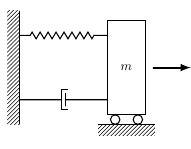
\includegraphics[width=\picwid]{massa_molla_smorzatore_HQ}
 % massa_molla_smorzatore_HQ.png: 0x0 px, 0dpi, 0.00x0.00 cm, bb=
 \label{fig:massa_molla_smorzatore_HQ}
\end{figure}

Si vuole costruire il modello ISU dell'oggetto.
Il corpo ha un solo grado di libertà, si fissa un sistema di riferimento.
Si indica con $s$ la posizione dell'oggetto.

Esistono due modalità principali per scrivere le equazioni di un sistema
meccanico, l'approccio Newtoniano e l'approccio Lagrangiano, si usa in seguito
quello Newtoniano.

Si applica il secondo principio delle dinamica, ossia le formule
precedentemente analizzate.

$$
m\ddot{s} = f - ks - b\dot{s}
$$
$(s_1 , \dot{s}_1 = 0)$

Il numero di equazioni da scrivere è pari al numero di masse moltiplicate per i
rispettivi gradi di libertà.

Le variabili del sistema sono
$$\begin{matrix}
f & s \\
(0) & (2) \\
f & s & \dot{s}\\
u & x_1 &x_2
\end{matrix}$$

Il sistema è del secondo ordine.
$$\left\{\begin{aligned}
\dot{x}_1 &= \dot{s} = x_2 \\
\dot{x}_2 &= \ddot{s} = \frac{1}{m}f - \frac{k}{m}s - \frac{b}{m}s =
-\frac{k}{m}x_1 - \frac{b}{m}x_2 + \frac{1}{m}u
\end{aligned}\right.$$

Le uscite saranno assegnate arbitrariamente, il sistema è lineare
tempo invariante e strettamente causale.

\end{document}
